\chapter{}
What exactly is a wavelet? A wavelet means a small wave. This term says a lot about it nature. Wavelets are a family of functions which oscillates like wave and should be compactly supported. Additionally, the wavelet has zero mean.

\begin{defn}
Wavelets are created by scaling and shifting of the, so called, mother wavelet $\psi(t)$. The child wavelets are defined as

\begin{equation}
\label{eq:wavelets}
\psi^{(a,b)}(t)=|a|^{-\frac{1}{2}} \psi\left(\frac{t-b}{a}\right),\ a>0. 
\end{equation}

\end{defn}


There are plenty of different mother wavelets, for example

\begin{figure}[h]
	\centering
	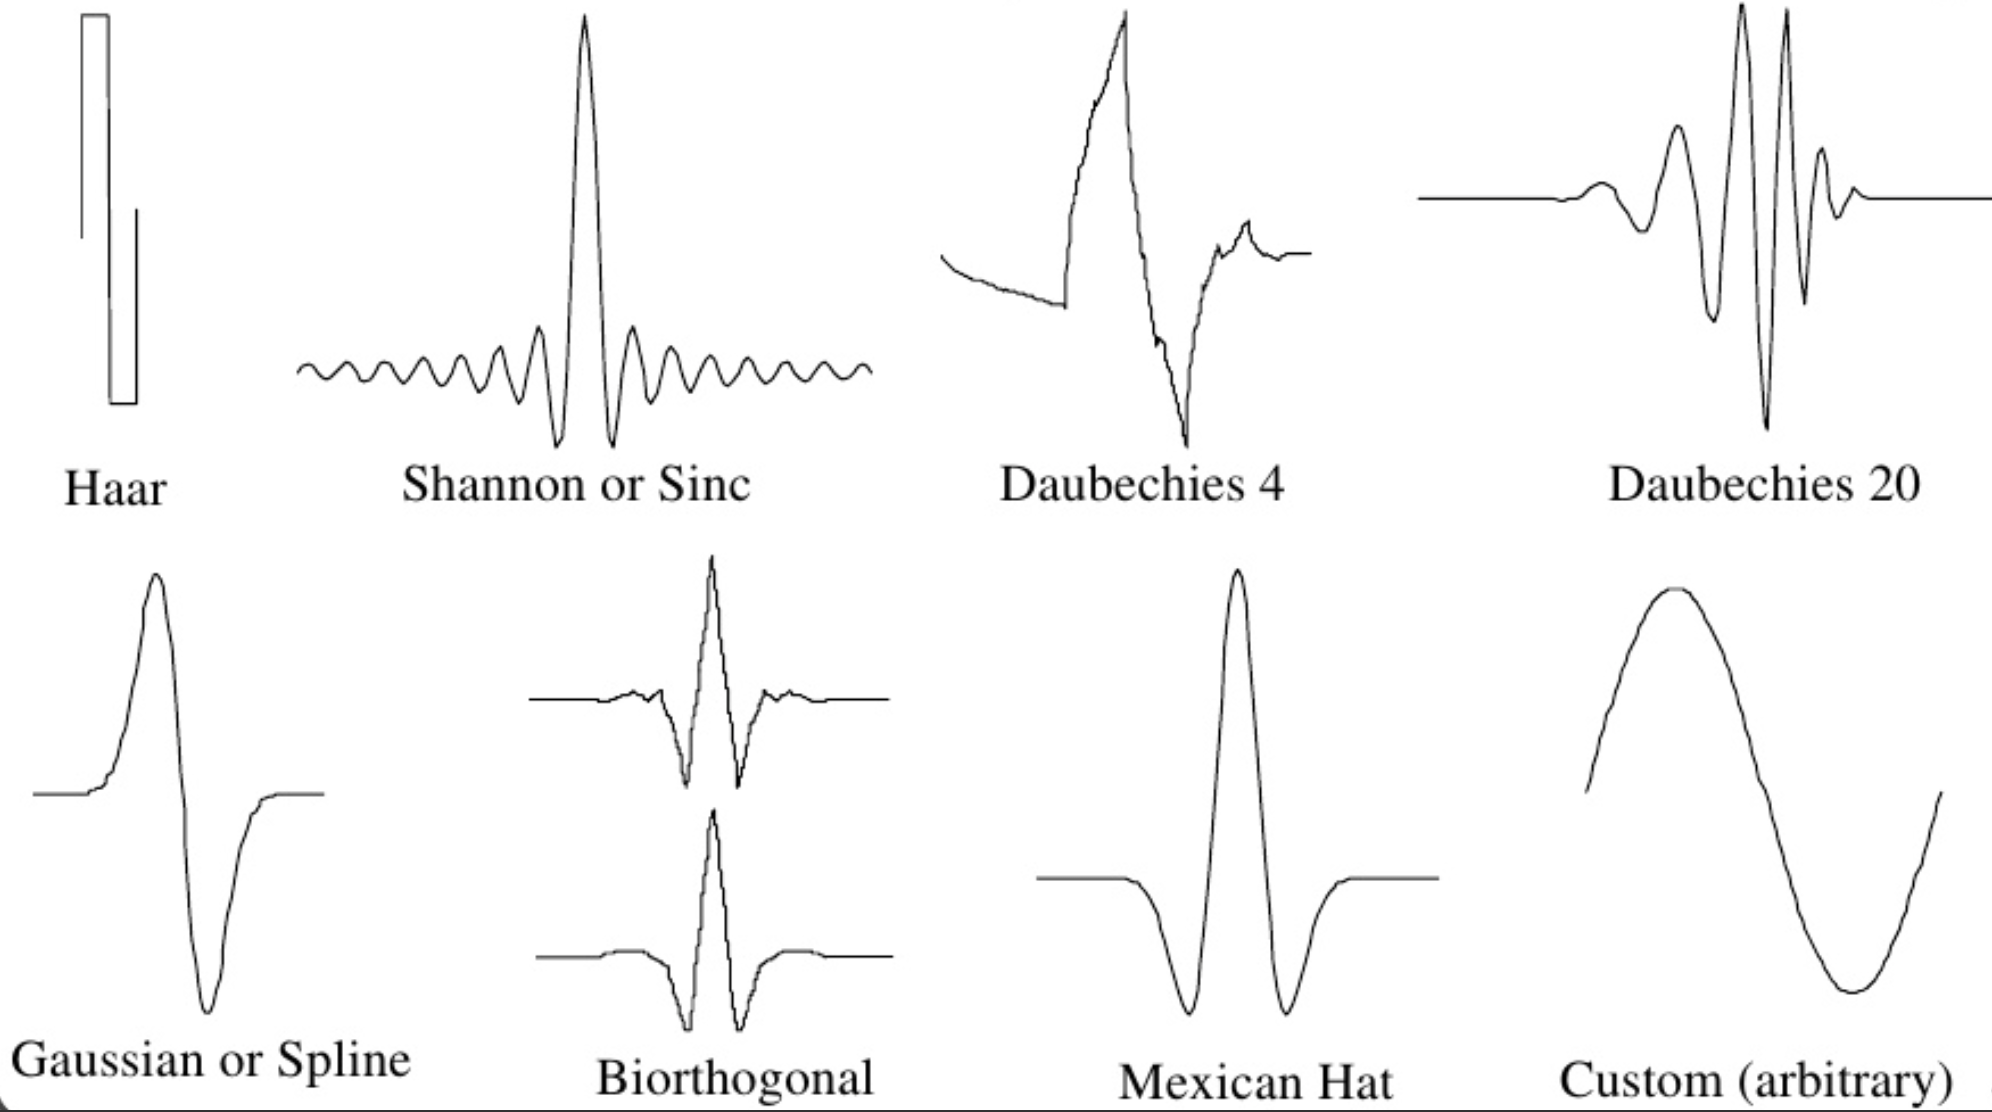
\includegraphics[width=\textwidth]{wavelets_with_bottom_line.png}
	\caption{Different types of wavelets.}
	\label{fig:wavelets}
\end{figure}

\textit{** Add more about wavelets properties? **}


\section{Daubechies wavelets}

Each type of wavelet function is more suitable for different applications. The best for image analysis are the Daubechies wavelets. 

\begin{defn}
Daubechies wavelets are collection of orthogonal and compactly supported functions. A denotation for those wavelets is $dbN$, where $N$ means a maximal number of vanishing moments.
\end{defn}

\begin{figure}[h]
	\centering
	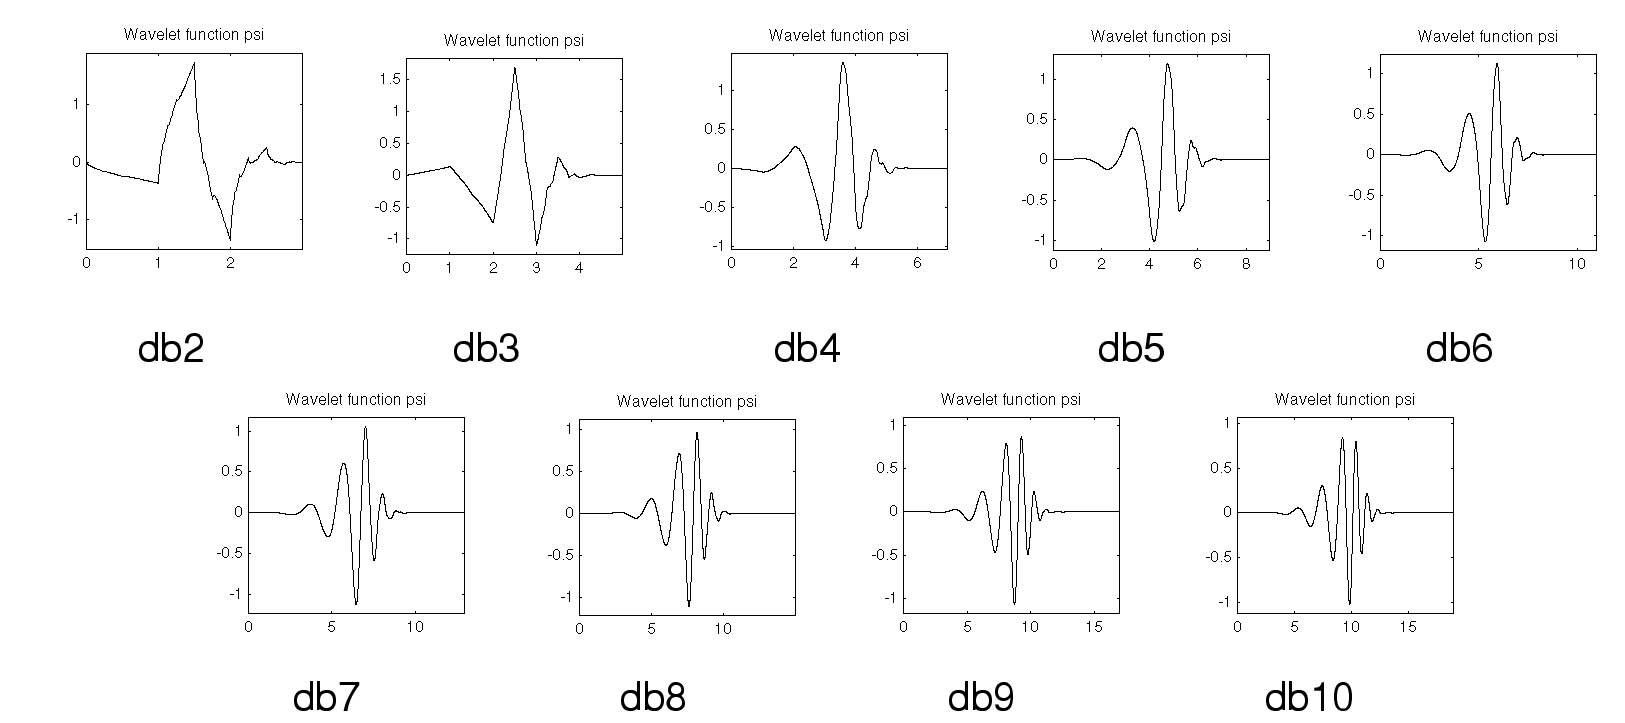
\includegraphics[width=\textwidth]{DB_N.png}
	\caption{Daubechies wavelets.}
	\label{fig:db_wavelets}
\end{figure}

\section{Wavelet Transform}

\textit{** Add some short introduction? **}

\begin{defn}
Wavelet transform

\begin{equation}
W(a,b)=\int_{-\infty}^{\infty} y(t) a^{-\frac{1}{2}} \psi\left(\frac{t-b}{a}\right) dt,
\end{equation}

where $a$ is scale parameter, $b$ translation parameter and $y(t)$ original signal.
\end{defn}

\subsection{Wavelet transform vs Fourier transform}

\begin{defn}
Fourier transform

\begin{equation}
Y(f)=\int_{-\infty}^{\infty} y(t) e^{-i\omega t} dt,
\end{equation}

where $y(t)$ is time domain signal and $Y(f)$ is frequency domain signal.
\end{defn}

\begin{table}[h]
\centering

\label{The diferrences between Wavelet Transform and Fourier Transform.}
\begin{tabular}{|p{0.5\linewidth}|p{0.5\linewidth}|}
\toprule
\textbf{ Wavelet transform} & \textbf{Fourier transform}
\\ \midrule
Suitable for stationary and non-\allowbreak -stationary signals 
& Suitable for stationary signals 
\\ \midrule
High time and frequency resolution
& Zero time resolution and very high frequency resolution     
\\ \midrule
Very suitable for studying the local behaviours of the signal
& No suitable  
\\ \midrule
Sine and cosine waves
& Scaled and translated mother wavelets
\\ \bottomrule
\end{tabular}
\end{table}

What differs both transformations is the type of function. In Fourier case there are sine and cosine functions, wherein wavelet transform uses wavelets.

Why use the Wavelet transform?
Sine function oscillates on the whole real axis, thus it cannot represent abrupt changes. However, the Wavelet transform is localized in space and time, so it can be used to detect sudden changes in signals and images. Moreover, wide range of wavelet functions is a main advantage of wavelet analysis.

\section{Discrete Wavelet transform}
There are two types of the wavelet transform:
\begin{itemize}
\item Continuous Wavelet Transform (CWT),
\item Discrete Wavelet Transform (DWT).
\end{itemize}

DWT is used to denoising and compression of signals and images. Also, DWT allows to detect smooth regions interrupted by edges or abrupt changes in contrast of images.

Scale and translation parameters are defined as

\begin{equation}
a = 2^j \text{ and } b = 2^j k,\ j,k=1,2,\ldots.
\end{equation}

to avoid redundancy in coefficients.


The figure \ref{fig:DWT} on a page \pageref{fig:DWT} shows how DWT works. Discrete Wavelet Transform splits signal with two filters: $h(n)$ - high pass filter (HPF) and $g(n)$ - low pass filter (LPF). The HPF captures a part with bigger frequencies which is the main signal. Whereas, the LPF captures smaller frequencies - a noise of the signal. Subsequently, both parts are down sampled by a factor of 2. This decomposition can be repeated on the HPF part of the signal. Hence, the next levels of DWT coefficients.

\begin{figure}[h]
	\centering
	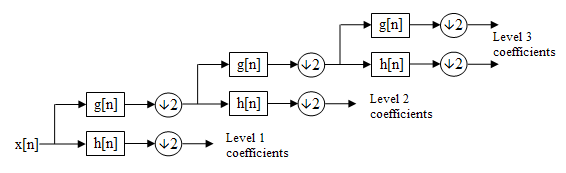
\includegraphics[width=\textwidth]{DWT.png}
	\caption{Discrete Wavelet transform on a signal $x(n)$.}
	\label{fig:DWT}
\end{figure}


\section{2-D Discrete Wavelet transform}

2-D Discrete Wavelet Transform works similar way as 1-D with High Pass Filter and Low Pass Filter, except that one level of the decomposition includes double filtering, on columns and rows. The figure \ref{fig:2D_DWT} shows image decomposition. Firstly, the DWT is applied on columns of the input image and then on the rows of the both outputs. Ultimately, there are four results:

\begin{itemize}
\item LL - result of LPF applied on both, columns and rows,
\item LH - result of LPF applied on columns and HPF on rows,
\item HL - result of HPF applied on columns and LPF on rows,
\item HH - result of HPF applied on both, columns and rows.
\end{itemize}  

\begin{figure}[h]
	\centering
	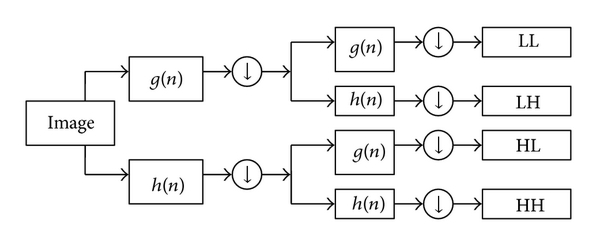
\includegraphics[width=\textwidth]{2D_DWT.JPG}
	\caption{2-D Discrete Wavelet transform on an image.}
	\label{fig:2D_DWT}
\end{figure}

Now lets focus on what exactly each result represent. First one, the LL is just an approximation of the image. Next, the LH shows abrupt changes in a horizontal direction, whereas the HL part present similar issues but in a vertical direction. The HH shows sudden changes in a diagonal direction. In conclusion, the output of 2-D DWT gives us an approximation of the image and three parts with abrupt changes in different directions. What information gives as these sudden variations? Thanks to those we are able to find a places where two smooth regions meets. This kind of image anomaly could be interpreted as edges.

\textit{** Explain what is an image approximation **}


